Let $u_1 \geq 0$ and $u_2 \geq 0$.This may be expressed as 
\begin{equation}
    \vec{u} = \myvec{u_1\\u_2} \geq 0
\end{equation}
From the given inequalities we have,
\begin{align}
   \myvec{2&1 \\ 1&2 }\vec{x} &\geq \myvec{8 \\ 10} \\
   \myvec{2&1 \\ 1&2 }\vec{x} - \vec{u} &= \myvec{8 \\ 10}
\end{align}

Now we have,
\begin{align}
\vec{x} &= \myvec{2 & 1 \\ 1 & 2}^{-1} \myvec{8 \\ 10} + \myvec{2 & 1 \\ 1 & 2}^{-1} \myvec{u_1 \\ u_2}\\
  \vec{x} &= \myvec{2\\4} + \frac{1}{3}\myvec{2 & -1 \\ -1 & 2}\myvec{u_1 \\ u_2} 
\end{align}

Thus the solution of the system of inequalities can be determined graphically and is represented in Fig.  \ref{ineq/52/fig1},
%
\begin{figure}[!ht]
    \centering
    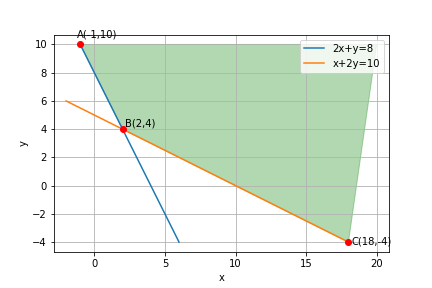
\includegraphics[width=\columnwidth]{solutions/su2021/2/52/assignment10.png}
    \caption{Graphical solution}
    \label{ineq/52/fig1}
\end{figure}

